% !TeX root = Bericht.tex
% !TeX spellcheck = en_US
\section{Experimental setup and procedure}\label{sec:procedure}
In this section, the experimental setup and all used components are described. The setup contains a laser diode with implemented temperature regulator. The laser beam gets redirected over two mirrors and enters a Fabry-Perot-Interferometer (FPI). This cavity consists of two parallel mirrors, whereby the rear mirror is moved forwards and backwards by a Piezo-Transducer. The setup is shown in \autoref{diodenlaser_aufbau_skript}. 

\begin{figure}[H]
	\centering
	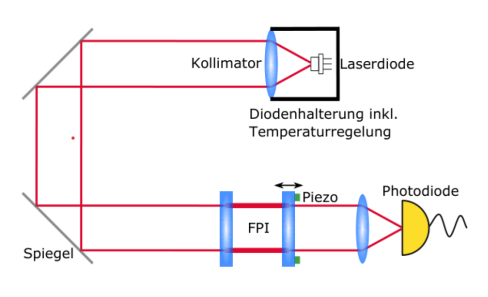
\includegraphics[ height=5cm]{versuchsaufbau}
	\caption{The experimental setup containing the laser diode, two deflecting mirrors, the FPI, with one mirror moved by a Piezo-transducer, and a photodiode afterwards. From \cite{diodenlaser}. }
	\label{diodenlaser_aufbau_skript} 
\end{figure}

In the first part, the emitted power of the laser beam is detected in dependence of the input-current. This measurement series is done for three different temperatures, $20 \unit{\degreeCelsius}$, $25 \unit{\degreeCelsius}$ and $30 \unit{\degreeCelsius}$. For each temperature, the current is varied from \SI{0}{mA} to \SI{35}{mA} in 21 steps. At currents below the threshold current we use steps of \SI{1}{mA}. When lasing starts up, steps of \SI{0.2}{mA} are used in order to accurately determine the threshold current. Afterwards, bigger steps are used again. For every current, the power is manually read off the powermeter. 

In the second part of the experiment, the frequency tuneability is being measured. Therefore, a triangle voltage is inserted at the Piezo-transducer, which is left unchanged during the experiment. The measured signal of the photodiode is saved onto an USB-stick from an oscilloscope connected to the photodiode. To explore the frequency tuneability dependent on current, three series of measurements are done at three temperatures, \SI{20}{\degreeCelsius}, \SI{25}{\degreeCelsius} and \SI{30}{\degreeCelsius}. In each case, the current is varied in 26 steps, starting at each threshold current that resulted from the first part of the experiment. Afterwards, the current is held constant at \SI{35.00(1)}{mA}. Now, the temperature is changed from \SI{20}{\degreeCelsius} to \SI{30}{\degreeCelsius} in steps of \SI{1}{\degreeCelsius}. It does not make sense to use smaller steps, as the screw that works as the temperature regulator does not provide higher resolution. 

%\begin{figure}[H]
%    \centering
%    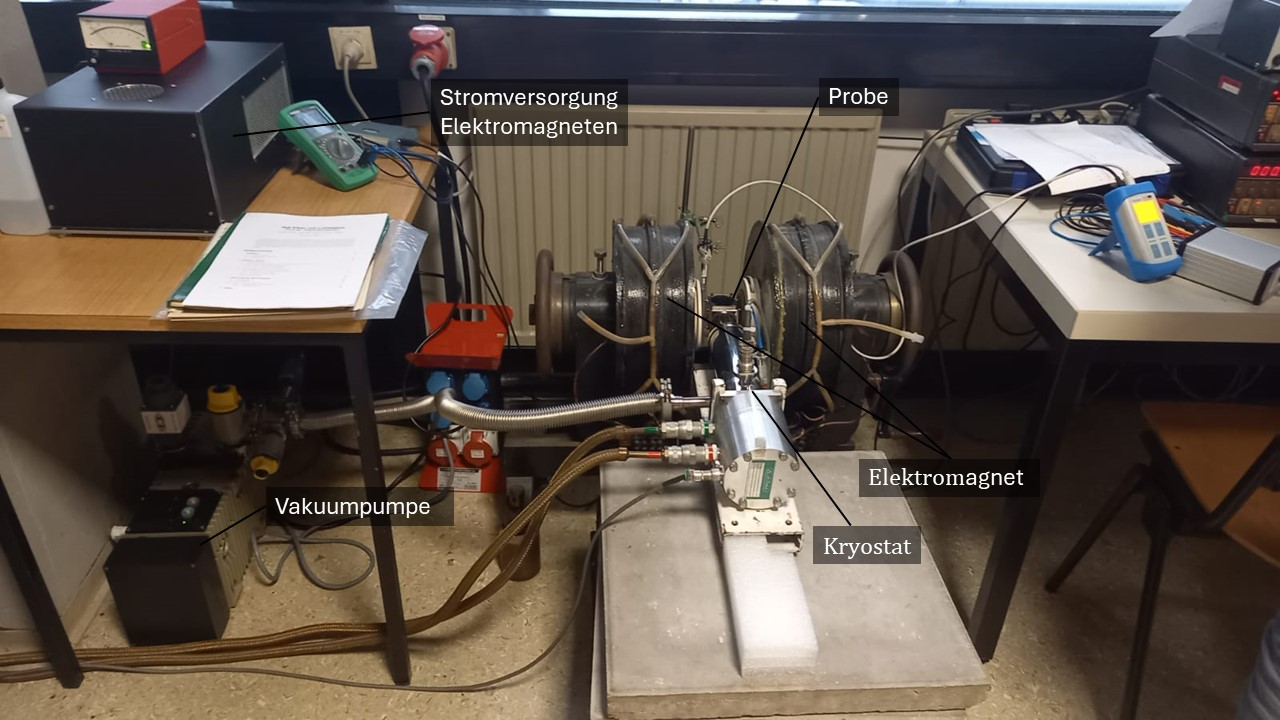
\includegraphics[width=\linewidth]{BildExberimentAufbauBeschriftung.JPG}
%    \caption{In dieser Abbildung sind der Kryostat, die Magnetspulen sowie die Sonde zur Messung des Magnetfeldes zu erkennen.}
%    \label{ExperimetAufbau}
%\end{figure}

